
\chapter{Nonlinear solution process} \label{ssn_nonlinear_solution_process}

All of the examples presented thus far have been linear equations.  For non-linear systems, the solution method described in \cref{ssn_galerkin_solve} no longer apply.  For these problems the $n$ unknown degrees of freedom of $u$---with vector representation $\rankone{u}$---may be uniquely determined by solving for the down gradient direction of a quadratic model of the functional \index{Residual} \emph{residual}
\begin{align}
  \label{nonlin_resid}
  \mathscr{R}(u) = 0,
\end{align}
formed by moving all terms of a variational form to one side of the equation.  The following sections explain two ways of solving problems of this nature.




%===============================================================================
\section{Newton-Raphson method} \label{ssn_newton_raphson}

One way to solve system \cref{nonlin_resid} is the \index{Newton-Raphson method} \emph{Newton-Raphson} method \citep{nocedal_2000}.  This method effectively linearizes the problem by first assuming an initial guess of the minimizer, $\rankone{u}_k$, and the functional desired to be minimized, $\mathscr{R}(\rankone{u}_k) = \mathscr{R}_k$, then uses the $\mathscr{R}$-intercept of the tangent line to this guess as a subsequent guess, $\rankone{u}_{k+1}$.  This procedure is repeated until either the absolute value of $\mathscr{R}$ is below a desired \emph{absolute tolerance} or the relative change of $\mathscr{R}$ between guesses $\rankone{u}_k$ and $\rankone{u}_{k+1}$ is below a desired \emph{relative tolerance} (\cref{nr_image}).

\begin{figure}
  \centering
    \def\svgwidth{\linewidth}
    \input{images/fenics_intro/svg/newton_raphson.pdf_tex}
  \caption[Newton-Raphson diagram]{Illustration of the Newton-Raphson method for solving \cref{nonlin_resid} for $u$.}
  \label{nr_image}
\end{figure}

\subsection{Procedure}

First, as elaborated upon by \citet{nocedal_2000}, the Taylor-series approximation of the residual $\mathscr{R}(\rankone{u}_k)$ perturbed in a direction $\rankone{p}_k$ provides a quadratic model $m_k(\rankone{p}_k)$,
\begin{align}
  \label{newton_quadradic_model}
  \mathscr{R}(\rankone{u}_k + \rankone{p}_k) &\approx \mathscr{R}_k + \rankone{p}_k\T \nabla \mathscr{R}_k + \frac{1}{2} \rankone{p}_k\T \nabla^2 \mathscr{R}_k \rankone{p}_k =: m_k(\rankone{p}_k).
\end{align}
Because we wish to find the search direction $\rankone{p}_k$ which minimizes $m_k(\rankone{p}_k)$, we set the gradient of this function equal to zero and solve
\begin{align}
  0 &= \nabla m_k(\rankone{p}_k) \notag \\
    &= \nabla \mathscr{R}_k + \nabla \left( \rankone{p}_k\T \nabla \mathscr{R}_k \right) + \nabla \left( \frac{1}{2} \rankone{p}_k\T \nabla^2 \mathscr{R}_k \rankone{p}_k \right) \notag \\
    \label{newton_zero_grad_condition}
    &= \nabla \mathscr{R}_k + \nabla^2 \mathscr{R}_k \rankone{p}_k,
\end{align}
giving us the \emph{Newton direction}
\begin{align}
  \label{newton_direction}
  \rankone{p}_k &= -\left( \nabla^2 \mathscr{R}_k \right)^{-1} \nabla \mathscr{R}_k.
\end{align}

Quadratic model \cref{newton_quadradic_model} is simplified to a linear model if the second derivative is eliminated.  Integrating \cref{newton_zero_grad_condition} over $\rankone{u}_k$ produces
\begin{align}
  \label{search_direction_equation}
  \nabla^2 \mathscr{R}_k \rankone{p}_k &= - \nabla \mathscr{R}_k \notag \\
  \int_{\rankone{u}_k} \nabla^2 \mathscr{R}_k(\rankone{u}_k) \rankone{p}_k \d{\rankone}{u}_k &= - \int_{\rankone{u}_k} \nabla \mathscr{R}_k(\rankone{u}_k) \d{\rankone}{u}_k \notag \\
  \nabla \mathscr{R}_k \rankone{p}_k &= - \mathscr{R}_k,
\end{align}
a discrete system of equations representing a first-order differential equation for Newton direction $\rankone{p}_k$.  To complete system \cref{search_direction_equation}, one boundary condition may be specified.  For all Dirichlet boundaries, $u$ is known and can therefore not be improved.  Hence search direction $p = 0$ over essential boundaries.  Boundaries corresponding to natural conditions of $u$ require no specific treatment.

The iteration with \emph{step length} or \emph{relaxation parameter} $\alpha \in (0,1]$ is defined as
\begin{align}
  \label{newton_iteration}
  \rankone{u}_{k+1} &= \rankone{u}_k + \alpha \rankone{p}_k.
\end{align}
Provided that the curve $\mathscr{R}$ is relatively smooth and that the Hessian matrix $\nabla^2 \mathscr{R}(\rankone{u}_k)$ in \cref{newton_direction} is positive definite, \cref{newton_iteration} describes an iterative procedure for calculating the minimum of $\mathscr{R}$ and corresponding optimal value of $\rankone{u}$.  See Algorithm \cref{newton_raphson_alg} and \CSLVR source code \cref{home_rolled_method} for details.

\subsection{G\^{a}teaux derivatives} \label{ssn_gateaux}

Because residual \cref{nonlin_resid} is a functional, \index{G\^{a}teaux derivative} \index{Directional derivative} \emph{G\^{a}teaux derivatives} are used to calculate the directional derivatives in \cref{search_direction_equation}.  To illustrate this derivative, consider the second-order boundary-value problem
\begin{align*}
  \nabla^2 u - u &= 0 &&\text{ in } \Omega \\
  \nabla u \cdot \rankone{n} &= g &&\text{ on } \Gamma.
\end{align*}
where $\Omega$ is the interior domain with boundary $\Gamma$, and $\rankone{n}$ is the outward-pointing normal vector.  The associated weak form is
\begin{align}
  \label{gateaux_example_form}
  \mathscr{R}(u) &= - \int_{\Omega} \nabla u \cdot \nabla \phi \d{\Omega} - \int_{\Omega} \phi u \d{\Omega} + \int_{\Gamma} \phi g \d{\Gamma} = 0,
\end{align}

The G\^{a}teaux derivative or first variation of $\mathscr{R}$ with respect to $u$ in the direction $p$---with vector notation $\delta_{\rankone{u}}^{\rankone{p}} \mathscr{R} (\rankone{u})$---is defined as
\begin{align*}
 \delta_{u}^{p}\mathscr{R}\left( u \right) = \frac{\delta}{\delta u} \mathscr{R}\left( u,p \right) = &\lim_{\epsilon \rightarrow 0} \totder{}{\epsilon} \mathscr{R} \left(u + \epsilon p \right) \\
  = &- \totder{}{\epsilon} \left[ \int_{\Omega} \nabla (u + \epsilon p) \cdot \nabla \phi \d{\Omega} \right]_{\epsilon = 0} \\
  &- \totder{}{\epsilon} \left[ \int_{\Omega} \phi (u + \epsilon p) \d{\Omega} \right]_{\epsilon = 0} \\
  &+ \totder{}{\epsilon} \left[ \int_{\Gamma} \phi g \d{\Gamma} \right]_{\epsilon = 0} \\
  = &- \int_{\Omega} \nabla p \cdot \nabla \phi \d{\Omega} - \int_{\Omega} \phi p \d{\Omega}.
\end{align*}
It is important to recognize that if $p$ is a function with known values, \ie data interpolated onto a finite-element mesh, the finite-element assembly---described in \cref{ssn_global_galerkin_assembly}---will result in a vector of length $n$.  However, if $p$ is an unknown quantity and thus a member of the trial space associated with the finite-element approximation of $\rankone{u}$, as is the case with the Newton-Raphson method here, the assembly process will result in a matrix with properties identical to the associated stiffness matrix of \cref{gateaux_example_form}.  In order to clearly differentiate between these circumstances, the G\^{a}teaux derivative operator notation $\delta_{\rankone{u}}^{\rankone{p}}$ is used when $\rankone{p}$ is a member of the trial space, and $\delta_{\rankone{u}}$ otherwise.

These derivatives may be calculated with FEniCS using the process of \index{Automatic differentiation} \emph{automatic differentiation} \citep{nocedal_2000}, as illustrated by the nonlinear problem example in \cref{river_cross_code}.

\begin{algorithm}
  \normalsize
  \begin{algorithmic}[1]
    \State \textbf{INPUTS}:
    \State \ \ \ $\phantom{a_{tol}}\mathllap{\mathscr{R}}$ - residual variational form
    \State \ \ \ $\phantom{a_{tol}}\mathllap{\rankone{u}}$ - initial state parameter vector
    \State \ \ \ $\phantom{a_{tol}}\mathllap{\hat{\rankone{p}}}$ - trial function in same space as $\rankone{u}$
    \State \ \ \ $\phantom{a_{tol}}\mathllap{\alpha}$ - relaxation parameter
    \State \ \ \ $a_{tol}$ - absolute tolerance to stop iterating
    \State \ \ \ $r_{tol}$ - relative tolerance to stop iterating
    \State \ \ \ $\phantom{a_{tol}}\mathllap{n_{max}}$ - maximum iterations
    \State \textbf{OUTPUT}:
    \State \ \ \ $\phantom{a_{tol}}\mathllap{\rankone{u}^*}$ - optimized state parameter vector
    \\
    \hrulefill
    \Function{NR}{$\mathscr{R},\ \rankone{u},\ \hat{\rankone{p}},\ \alpha,\ a_{tol},\ r_{tol},\ n_{max}$}
      \State $\phantom{\rankone{\vartheta}}\mathllap{r} := \infty$
      \State $\phantom{\rankone{\vartheta}}\mathllap{a} := \infty$
      \While{$(a > a_{tol}$ \textbf{or} $r > r_{tol})$ \textbf{and} $n < n_{max}$}
        \State $\phantom{\rankone{p}}\mathllap{J} :=$ \textbf{assemble} $\delta_{\rankone{u}}^{\hat{\rankone{p}}} \mathscr{R}(\rankone{u})$
        \State $\phantom{\rankone{p}}\mathllap{\rankone{b}} :=$ \textbf{assemble} $\mathscr{R}(\rankone{u})$
        \State $\phantom{\rankone{p}}\mathllap{\rankone{p}} \leftarrow$ \textbf{solve} $J \rankone{p} = -\rankone{b}$
        \State $\phantom{\rankone{p}}\mathllap{\rankone{u}} := \rankone{u} + \alpha \rankone{p}$
        \State $\phantom{\rankone{p}}\mathllap{a} := \Vert \rankone{b} \Vert_{2}$
        \If{$n = 0$}
          \State $a_0 := a$
        \EndIf
        \State $\phantom{\rankone{p}}\mathllap{r} := a / a_0$
        \State $\phantom{\rankone{p}}\mathllap{n} := n + 1$
      \EndWhile
    \State \Return $\rankone{u}^* := \rankone{u}$ 
    \EndFunction
  \end{algorithmic}
  \caption[Newton-Raphson]{ - Newton-Raphson method}
  \label{newton_raphson_alg}
\end{algorithm}

\pythonexternal[caption={Newton-Raphson method as implemented in \CSLVR's \texttt{model} class}, label = home_rolled_method, firstline=2073, lastline=2145]{cslvr_src/model.py}




%===============================================================================
\section{Nonlinear problem example}

\index{Non-linear differential equations!1D}
Suppose we would like to minimize the time for a boat to cross a river.  The time for this boat to cross, when steered directly perpendicular to the river's parallel banks is given by
\begin{align*}
  T(y) &= \int_0^T \d{t} = \int_0^S \totder{t}{s} \d{s} = \int_0^S \frac{1}{\Vert \rankone{u}\Vert} \d{s} \\
  T(y) &= \int_0^{\ell} \frac{\sqrt{1 + (y')^2}}{\Vert \rankone{u} \Vert} \d{x} \\
  T(y) &= \int_0^{\ell} \frac{\sqrt{1 + (y')^2}}{\sqrt{v^2 + u^2}} \d{x} = \int_0^{\ell} L(x,y') \d{x},
\end{align*}
where $S$ is the length of the boat's path; $\rankone{u}$ is the velocity of the boat with components river current speed $v(x)$ and boat speed $u$ in the $x$ direction as a result of its motor; and $\ell$ is the width of the river.  For \emph{Lagrangian} $L$, the first variation of $T$ in the direction of the test function $\phi \in \testspace$ (see test space \cref{test_space}) is
{\footnotesize
\begin{align*}
  \delta T(y,\phi) &= \totder{}{\epsilon} \int_0^{\ell} L(x, y + \epsilon \phi, y' + \epsilon \phi') \d{x} \Bigg|_{\epsilon = 0} \\
                   &= \int_0^{\ell} \left( L_y \phi + L_{y'} \phi' \right) \d{x} \\
                   &= \int_0^{\ell} \left( L_y - \totder{}{x} L_{y'} \right) \phi \d{x} + L_{y'} \phi \Big|_{x=0}^{x=\ell} \\
                   &= \int_0^{\ell} \left( L_y - \left[ L_{y'x} + L_{y'y} y' + L_{y'y'} y'' \right] \right) \phi \d{x} + L_{y'} \phi \Big|_{x=0}^{x=\ell}.
\end{align*}}
Evaluating each individual term,
\begin{align*}
  L_y          &= 0 \\
  L_{y'}(y')   &= \frac{y' \left(1 + (y')^2\right)^{-1/2}}{\sqrt{v^2 + u^2}} \\
  L_{y'x}(y')  &= \frac{\left(2(y')^2 + 1\right) y''}{\sqrt{u^2 + v^2} \sqrt{1 + (y')^2}} \\
  L_{y'y}      &= 0 \\
  L_{y'y'}(y') &= \frac{1}{\sqrt{u^2 + v^2} \sqrt{1 + (y')^2}} \left( 1 - \frac{(y')^2}{\left(1 + (y')^2\right)^3} \right),
\end{align*}
and so the first variation of $T$ is reduced to
\begin{align}
  \label{boat_T_fv}
  \delta T(y,\phi) &= - \int_0^{\ell} \left( L_{y'x} + L_{y'y'} y'' \right) \phi \d{x} + L_{y'} \phi \Big|_{x=0}^{x=\ell}.
\end{align}
In order to find the minimal time for the boat to cross, this first variation of $T$ must to be equal to zero.  First, defining
\begin{align*}
  M &= \frac{L_{y'x}}{y''},
\end{align*}
relation \cref{boat_T_fv} can be rewritten followed by integrating by parts of the the second-derivative term once again,
{\footnotesize
\begin{align*}
  0 &= - \int_0^{\ell} \left( M y'' + L_{y'y'} y'' \right) \phi \d{x} + L_{y'} \phi \Big|_{x=0}^{x=\ell} \\
    &= - \int_0^{\ell} \left( M + L_{y'y'} \right) y'' \phi \d{x} + L_{y'} \phi \Big|_{x=0}^{x=\ell} \\
    &= \int_0^{\ell} \left( M + L_{y'y'} \right) y' \phi' \d{x} - \left[ M + L_{y'y'} \right] y' \phi \Big|_{x=0}^{x=\ell} + L_{y'} \phi \Big|_{x=0}^{x=\ell}.
\end{align*}}
If the left essential boundary condition is set to $y(0) = 0$, and the right natural boundary condition is set to be equal to the trajectory of the boat at the opposite bank given by
$$y'(\ell) = g = \frac{v(\ell)}{u},$$
the final variational problem therefore consists of finding $y \in \trialspace$ (see trial space \cref{trial_space}) such that
{\tiny
\begin{align*}
  0 &= \int_0^{\ell} \left( M(y') + L_{y'y'}(y') \right) y' \phi' \d{x} - \left[ M(g) + L_{y'y'}(g) \right] g \phi \Big|_{x=\ell} + L_{y'}(g) \phi \Big|_{x=\ell}.
\end{align*}}
for all $\phi \in \testspace$.

The weak solution to this equation using linear-Lagrange shape functions \cref{linear_lagrange_functions} using the built-in FEniCS Newton solver is shown in \cref{river_cross_image} and generated from \cref{river_cross_code}.

\pythonexternal[label=river_cross_code, caption={FEniCS source code for the river crossing example.}]{scripts/fenics_intro/river_cross.py}

\begin{figure}
  \centering
    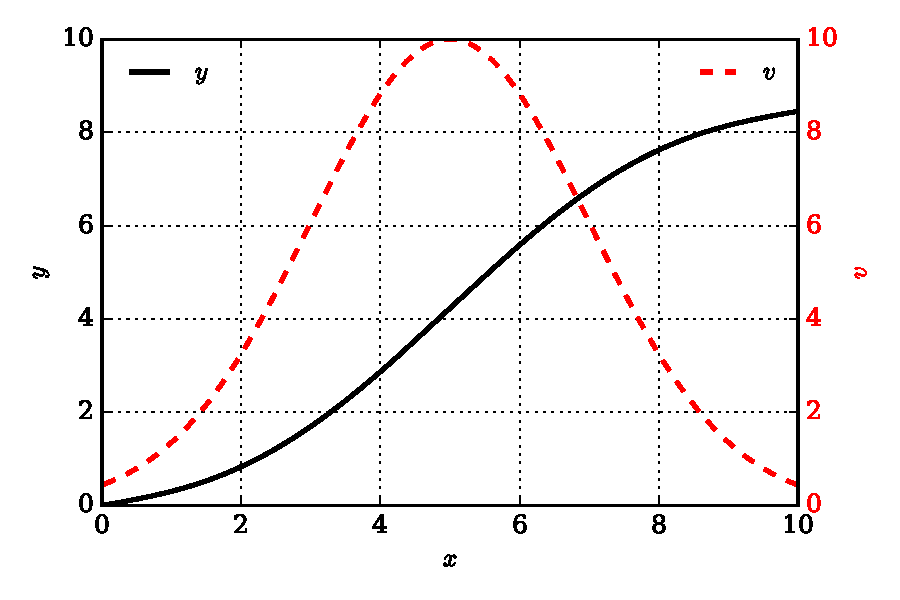
\includegraphics[width=\linewidth]{images/fenics_intro/river_cross.pdf}
  \caption[Nonlinear problem example]{Path taken for a boat to cross a river, $y(x)$ (solid black), with a motor speed in the $x$-direction of $u = 1$, and river velocity in the $y$-direction $v(x)$ (dashed red).}
  \label{river_cross_image}
\end{figure}




%===============================================================================
\section{Quasi-Newton solution process}

\index{Quasi-Newton methods}
In some situations, full quadratic model \cref{newton_quadradic_model} may be preferred over linear model \cref{search_direction_equation} for solving a non-linear system.  When the inverse of Hessian matrix $\nabla^2 \mathscr{R}_k$ is difficult to calculate by hand, it may be approximated by using curvature information at a current guess $\rankone{u}_k$.  Algorithms utilizing the Hessian approximation are referred to as \emph{quasi-Newton} methods.

\index{BFGS Algorithm}
As described by \citet{nocedal_2000}, the most modern and efficient of such Hessian approximation techniques is that proposed by Broyden, Fletcher, Goldfarb, and Shanno, aptly referred to as the BFGS method (Algorithm \cref{BFGS_alg}).  This method uses the iteration
\begin{align}
  \label{qn_iteration}
  \rankone{u}_{k+1} = \rankone{u}_k + \alpha_k \rankone{p}_k
\end{align}
and a quadratic model similar to \cref{newton_quadradic_model} with the addition of a subsequent iteration $k+1$ quadratic model:
\begin{align}
  \label{qn_k_quadradic_model}
  m_{k}(\rankone{p}) &= \mathscr{R}_{k+1} + \rankone{p}\T \nabla \mathscr{R}_{k} + \frac{1}{2} \rankone{p}\T B_{k} \rankone{p} \\
  \label{qn_k+1_quadradic_model}
  m_{k+1}(\rankone{p}) &= \mathscr{R}_{k+1} + \rankone{p}\T \nabla \mathscr{R}_{k+1} + \frac{1}{2} \rankone{p}\T B_{k+1} \rankone{p}.
\end{align}
The minimizer of \cref{qn_k_quadradic_model}, search direction $\rankone{p}_k$, is found identically to Newton direction \cref{newton_direction}:
\begin{align*}
  \rankone{p}_k &= - B_k^{-1} \nabla \mathscr{R}_k,
\end{align*}
where the approximate Hessian matrix $B_k \approx \nabla_{\rankone{u} \rankone{u}}^2 \mathscr{R}_k$ must be symmetric and positive definite.  Furthermore, it is required that $\nabla m_{k+1} = \nabla \mathscr{R}_j$ for $j = k, k+1$, the last two iterates.  For the last iterate $k+1$, $\mathscr{R}_{k+1}$ is evaluated at $\rankone{u}_{k+1}$ and therefore the gradient of $m_{k+1}$ at $\rankone{p} = \rankone{0}$ is evaluated,
\begin{align*}
  \nabla m_{k+1}(\rankone{0}) &= \nabla \mathscr{R}_{k+1},
\end{align*}
implying that the second condition is satisfied automatically.  Using the same reasoning and iteration \cref{qn_iteration}, to evaluate $m_{k+1}$ at $\rankone{u}_{k}$ the gradient of $m_{k+1}$ at $\rankone{p} = -\alpha_k \rankone{p}_k$ is evaluated,
\begin{align*}
  \nabla m_{k+1}(-\alpha_k \rankone{p}_{k}) &= \nabla \mathscr{R}_{k+1} - \alpha_k \rankone{p}_{k} B_{k+1} = \nabla \mathscr{R}_k,
\end{align*}
thus requiring that
\begin{align*}
  \alpha_k \rankone{p}_k B_{k+1} &= \nabla \mathscr{R}_{k+1} - \nabla \mathscr{R}_k.
\end{align*}
Using iteration \cref{qn_iteration}, the \index{Secant equation} \emph{secant equation} is
\begin{align}
  \label{secant_equation}
  B_{k+1} \rankone{s}_k &= \rankone{y}_k,
\end{align}
where
\begin{align*}
  \rankone{s}_k = \rankone{u}_{k+1} - \rankone{u}_k \hspace{10mm} \rankone{y}_k &= \nabla \mathscr{R}_{k+1} - \nabla \mathscr{R}_k.
\end{align*}
Equivalently, the \emph{inverse secant equation} is
\begin{align}
  \label{inverse_secant_equation}
  H_{k+1} \rankone{y}_k &= \rankone{s}_k,
\end{align}
where $H_{k+1} = B_{k+1}^{-1}$.

As described by \citet{nocedal_2000}, inverse secant equation \cref{inverse_secant_equation} will be satisfied if the \emph{curvature condition}
\begin{align*}
  \rankone{s}_k\T \rankone{y}_k > 0
\end{align*} 
holds.  This is explicitly enforced by choosing step length $\alpha_k$ in \cref{qn_iteration} such that the \index{Armijo condition} \emph{Armijo condition}
\begin{align}
  \label{armijo_condition}
  \mathscr{R}(\rankone{u}_k + \alpha_k \rankone{p}_k ) \leq \mathscr{R}_k + c_1 \alpha_k \rankone{p}\T \nabla \mathscr{R}_k
\end{align}
and the curvature condition 
\begin{align}
  \label{curvature_condition}
  \rankone{p}\T \nabla \mathscr{R}(\rankone{u}_k + \alpha_k \rankone{p}_k ) \geq c_2 \rankone{p}\T \nabla \mathscr{R}_k,
\end{align}
collectively referred to as the \index{Wolfe conditions} \emph{Wolfe conditions}, hold for some pair of constants $c_1,c_2 \in (0,1)$.
One way of enforcing \cref{armijo_condition,curvature_condition} is described by the \index{Backtracking line search} \emph{backtracking line search}, Algorithm \cref{qn_bls_alg} \citep{nocedal_2000}.

In order to derive a unique $H_{k+1}$, the additional constraint that $H_{k+1}$ be close to the current matrix $H_k$ is imposed.  Thus $H_{k+1}$ is the solution to the problem
\begin{align}
  \label{qn_H_problem}
  \min_{H} \Vert H - H_k \Vert
\end{align}
\begin{align}
  \label{qn_H_problem_constraints}
  \text{subject to} \hspace{5mm} H = H\T, \hspace{5mm} H \rankone{y}_k = \rankone{s}_k.
\end{align}
Using the weighted \emph{Frobenius} norm
\begin{align*}
  \Vert A \Vert_W = \left\Vert W^{\nicefrac{1}{2}} A W^{\nicefrac{1}{2}} \right\Vert_F
\end{align*}
with average Hessian inverse
\begin{align*}
  W = \left[ \int_0^1 \nabla^2 \mathscr{R}(\rankone{u} + \tau \alpha_k \rankone{p}_k ) \d{\tau} \right]^{-1}
\end{align*}
satisfying $W\rankone{y}_k = \rankone{s}_k$ in \cref{qn_H_problem} gives the unique solution to \cref{qn_H_problem,qn_H_problem_constraints}
{\footnotesize
\begin{align*}
  H_{k+1} &= \left( I - \rankone{\rho}_k \rankone{s}_k \rankone{y}_k\T \right) H_k \left( I - \rho_k \rankone{y}_k \rankone{s}_k\T \right) + \rho_k \rankone{s}_k \rankone{s}_k\T, \hspace{5mm} \rho = \left( \rankone{y}\T \rankone{s} \right)^{-1}.
\end{align*}}

The iterative process for this method is described by Algorithm \cref{BFGS_alg}.

\begin{algorithm}
  \normalsize
  \begin{algorithmic}[1]
    \State \textbf{INPUTS}:
    \State \ \ \ $\phantom{a_{tol}}\mathllap{\rankone{u}}$ - initial state parameter vector
    \State \ \ \ $\phantom{a_{tol}}\mathllap{H}$ - inverse Hessian approximation
    \State \ \ \ $a_{tol}$ - absolute tolerance to stop iterating
    \State \ \ \ $r_{tol}$ - relative tolerance to stop iterating
    \State \textbf{OUTPUT}:
    \State \ \ \ $\phantom{a_{tol}}\mathllap{\rankone{u}^*}$ - optimized state parameter vector
    \\
    \hrulefill
    \Function{BFGS}{$\rankone{u},\ H,\ a_{tol}$}
      \State $\phantom{\rankone{\vartheta}}\mathllap{r} := \infty$
      \State $\phantom{\rankone{\vartheta}}\mathllap{a} := \infty$
      \While{$a > a_{tol}$ \textbf{or} $r > r_{tol}$}
        \State $\phantom{\rankone{p}}\mathllap{\rankone{g}} :=$ \textbf{assemble} $\delta_{\rankone{u}} \mathscr{R}(\rankone{u})$
        \State $\rankone{p} := - H \rankone{g}$
        \State $\phantom{\rankone{p}}\mathllap{\alpha} :=$ BLS$(\rankone{p}, \rankone{g}, \rankone{u})$
        \State $\phantom{\rankone{p}}\mathllap{\rankone{u}_k} := \rankone{u} + \alpha \rankone{p}$
        \State $\phantom{\rankone{p}}\mathllap{\rankone{g}_k} :=$ \textbf{assemble} $\delta_{\rankone{u}} \mathscr{R}(\rankone{u}_k)$
        \State $\phantom{\rankone{p}}\mathllap{\rankone{s}} := \rankone{u}_k - \rankone{u}$
        \State $\phantom{\rankone{p}}\mathllap{\rankone{y}} := \rankone{g}_k - \rankone{g}$
        \State $\phantom{\rankone{p}}\mathllap{\rho} := \left( \rankone{y}\T \rankone{s} \right)^{-1}$
        \State $\phantom{\rankone{p}}\mathllap{H} := \left( I - \rankone{\rho} \rankone{s} \rankone{y}\T \right) H \left( I - \rho \rankone{y} \rankone{s}\T \right) + \rho \rankone{s} \rankone{s}\T$
        %\State $\phantom{\rankone{p}}\mathllap{B} := B - \frac{B \rankone{s} \rankone{s}\T B}{\rankone{s}\T B \rankone{s}} + \frac{\rankone{y} \rankone{y}\T}{\rankone{y}\T \rankone{s}}$
        \State $\phantom{\rankone{p}}\mathllap{a} := \Vert \rankone{g}_k \Vert_{\infty}$
        \State $\phantom{\rankone{p}}\mathllap{r} := \Vert \rankone{u} - \rankone{u}_k \Vert_{\infty}$
        \State $\phantom{\rankone{p}}\mathllap{\rankone{u}} := \rankone{u}_k$
      \EndWhile
    \State \Return $\rankone{u}^* := \rankone{u}$ 
    \EndFunction
  \end{algorithmic}
  \caption[BFGS]{ - BFGS quasi-Newton method}
  \label{BFGS_alg}
\end{algorithm}

\begin{algorithm}
  \normalsize
  \begin{algorithmic}[1] 
    \State \textbf{INPUTS}:
    \State \ \ \ $\rankone{p}$ - search direction
    \State \ \ \ $\rankone{g}$ - vector assembly of $\delta_{\rankone{u}} \mathscr{R}$
    \State \ \ \ $\phantom{\rankone{p}}\mathllap{\rankone{u}}$ - state parameter vector
    \State \textbf{OUTPUT}: 
    \State \ \ \ $\phantom{\rankone{p}}\mathllap{\alpha}$ - Step length.
    \\
    \hrulefill
    \Function{BLS}{$\rankone{p},\ \rankone{g},\ \rankone{u}$}
      \State $\phantom{\ell_k}\mathllap{\alpha} := 1, \hspace{3mm} c_1 := 10^{-4}, \hspace{3mm} c_2 := \nicefrac{9}{10}$
      \State $\phantom{\ell_k}\mathllap{\ell_0} := $ \textbf{assemble} $\mathscr{R}\left( \rankone{u} \right)$
      \State $\ell_k := $ \textbf{assemble} $\mathscr{R}\left( \rankone{u} + \alpha \rankone{p} \right)$
      \While{$\ell_k \geq \ell_0 + c_1 \alpha \rankone{g}\T \rankone{p}$}
        \State $\phantom{\ell_k}\mathllap{\alpha} := c_2 \alpha$
        \State $\ell_k := $ \textbf{assemble} $\mathscr{R}\left( \rankone{u} + \alpha \rankone{p} \right)$
      \EndWhile
      \State \Return $\alpha$
    \EndFunction
  \end{algorithmic}
  \caption[Backtracking line-search]{ - Backtracking line search}
  \label{qn_bls_alg}
\end{algorithm}
